% formatar melhor essa parte. esta muito confusa e nao ha resultados tangiveis que influenciem na bateria para serem discutidos. 


Alternatively, the use of a NACA inlet can be considered, as follows.

\subsubsection{NACA inlet}
For a drag generated by a NACA inlet, a empirical method described by Silveira(2017) will be used, with the same characteristics of your inlet. It consists in use of a ESDU(Engineering Science Database Unit) - 1986. This method utilize a catalogued database to compute the drag and pressure recovery of air inlets totally or partially immersed in the boundary layer to predict and calculate the parameters from the inlet. The figure 3 show how it method works.

\begin{figure}
     \centering
     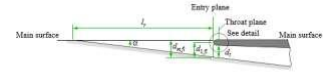
\includegraphics{fig/ESDU.png}
     \caption{Scheme and parameters of the inlet designed - ESDU, 1986}
     \label{fig:conduction}
 \end{figure}

How this method utilize the theory of two-dimensional boundary-layer calculation is used as reference, just in case of subsonic speeds this approach could be applied. 

For a curved-divergent ramp inlet operating at maximum efficiency – Fig. 4, once given initial conditions to the problem it is calculated the mass flow parameter by
equation (18):

\begin{equation}
     \frac{\frac{dm}{dt}}{ \rho V \theta^2 } = \dfrac{\frac{dm}{dt}}{1,121x61,73x0,003048^2}
\end{equation}


Where


\begin{math}
\frac{dm}{dt} - mass flow (kg/s);

{\rho} - air density (kg/m^3);

V - Speed of Airplane (m/s);

\theta - distance in plate (m);

\end{math}


Utilizing a throat aspect ratio of w/diamthroat = 4 and using the figure 20 (from ESDU, 1986) for a sizing a inlet to operate at maximum ram pressure efficiency, it was found:

\begin{equation}
    \frac{\theta}{diamthroat} = 0.075\\
\end{equation}

The boundary layer momentum thickness founded is \begin{math} \theta = 0.002358 \end{math}. Then, the value of diamthroat is 0.03144 m. With the value of throat diameter, it is possible to get the width, from throat aspect ratio:

\begin{equation}
    w = diamthroat*4 = 0.12576 m
\end{equation}

Following Silveira(2017), the method assume that the lip is calculated assuming elliptically rounded with the lip length and thickness in the throat plane both equal to a quarter of the throat diameter in equation (21):

\begin{equation}
    l = t = 0.25*diamthroat\\
    t = 0.25*0.03144 = 0.00786\\ 
\end{equation}

For the maximum external height of the inlet, \begin{math} d_{mfl} \end{math} and the lip highlight height, \begin{math} d_{1fl} \end{math}, determined in the inlet plane relative to ramp floor, are calculated by equations (22) and (23):

\begin{equation}
    d_{mfl} = diamthroat + t - l_1*tan(\alpha) = 0.03377
\end{equation}

\begin{equation}
d_{1fl} = diamthroat + 0.5t - l_1*tan(\alpha) = 0.02984
\end{equation}

The inlet capture area \begin{math} A_{inlet} \end{math} is given for:

\begin{equation}

A_{inlet} = w*d_{1fl} = 0.12576*0.02984 = 0.00375 m^2

\end{equation}

The maximum ram pressure efficiency, for the considerated values for the inlet, like the ramp angle equal a 7 and a throat aspect ratio of 4 is function of \begin{math} \frac{\theta}{diamthroat} \end{math} , the maximum ram pressures obtained from fig.17 (ESDU, 1986) is 0.82. From fig. 18 (ESDU,1986), it is possible to find the mass flow ratio at this value of efficiency as Mm = 0.425, using equation (14) it can be found the following ratio:

\begin{equation}
   \frac{\frac{dm}{dt}}{\frac{dm}{dt}_0} = 0.475*\frac{diamthroat}{d_{1fl}} =  0.475*\frac{0.03144}{0.02984} = 0.500
\end{equation}
 
The total drag coefficient is a sum from three components of drag: ram drag, spillage drag and incremental drag correction, which is described in the equation (27):

\begin{equation}
    C_{dfl} = 2*K_{fl}*\frac{\frac{dm}{dt}}{\frac{dm}{dt}_0} + k_{\alpha}*k_{M}*k_{spfl}*C_{Dfl}^{'} + \Delta C_D
\end{equation}

The value of \begin{math} K_{fl} \end{math} will be calculated from equation (16), and the factor \begin{math} k_{\psi} = 1 \end{math}:

\begin{equation}
    K_{fl} = k_{\psi}*\frac{\psi_{T}}{\psi_{0}}
\end{equation}

Utilizing figure 2(ESDU,1986), the momentum flow could be find through of the values of \begin{math} \frac{\delta}{d_{lfl}} \end{math} and M. Thus, the ram drag component could be find next:

\begin{equation}
     2k_{\psi}*\frac{\psi_{T}}{\psi_{0}}*\frac{\frac{dm}{dt}}{\frac{dm}{dt}_0} = 0.845
\end{equation}

From the fig. 12, 13 and 14 of ESDU (1986), the values of factors \begin{math}  k_{\alpha}, k_{M}, k_{spfl}* \end{math}, respectively can be found:

\begin{math}
 k_{\alpha} = 1
 k_{M} = 1 
 k_{spfl} = 0.1793
 \end{math}
The last term of spillage drag coefficient can be find through of fig. 11 (ESDU) for a curved-divergent ramp and as a function of \begin{math} d_{mfl}-d_{lfl}/l_{l} \end{math}. Thus:

\begin{math}
 k_{\alpha}*k_{M}*k_{spfl}*C_{Dfl}^{'} = 0.0287
 
\end{math}  

For the incremental drag correction, fig. 15 (ESDU) will be utilized as a function of mass flow ratio founded in equation (26). Then:

\begin{math}
\Delta C_D = 0.0017
\end{math}

Summing the three terms founded in equation (26), the total drag in air-intake can be given:

\begin{math}
C_{dfl} = 0.875
\end{math}

The final geometry of NACA inlet can be seen in figure 5.

\begin{figure}
     \centering
     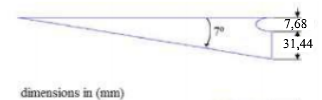
\includegraphics{fig/modelled.png}
     \caption{Lateral view of NACA Air Inlet}
     \label{fig:modelled}
 \end{figure}